\chapter*{Cryptographically-secure passphrases with Diceware}
\label{ch:diceware}

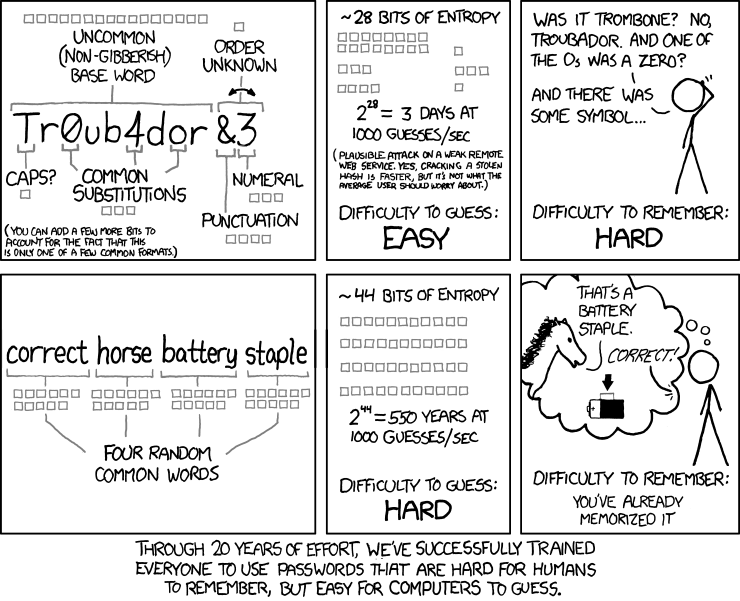
\includegraphics[width=\textwidth]{password_strength.png}

\newpage
\small
\setlength{\parindent}{0em}
\setlength{\parskip}{0.5em}

\subsubsection*{What is a Diceware passphrase?}

A passphrase is a bunch of words and characters that you type in to your computer to let it know for sure that the person typing is you. Passphrases differ from passwords only in length.

Diceware is a method for picking passphrases that uses dice to select words at random from a special list. Each word in the list is preceded by a four digit number. All the digits are between one and six, allowing you to use the outcomes of four dice rolls to select a word from the list.

\subsubsection*{Directions}

\begin{itemize}[leftmargin=*]

\item[1] Decide how many words you want in your passphrase. A four-word passphrase provides a level of security \textit{much} higher than the passwords most people use. For NSA-proof security, use seven.

\item[2] Roll all four dice at once and write the results down, reading from left to right, on a scrap paper. Make as many of these four-digit groups as you want words in your passphrase.

\item[3] Flip to the word list and look up the corresponding word next to each four-digit number.

\item[4] The words that you have found are your new passphrase! If required, capitalize a memorable word, and replace the last word with its four digit number.

\item[5] Come up with a way to remember your phrase. It might be a story, scenario, or sentence that that can remind you of the particular words you chose, in order.

\end{itemize}

\subsubsection*{Example}

Suppose you want a five-word passphrase. You will need $5 \times 4$ or 20 dice rolls. Let's say they come out as:

1, 6, 6, 6, 5, 1, 5, 6, 5, 3, 5, 6, 3, 2, 2, 3, 5, 6, 2, and 6. 

Write the results on a scrap of paper in groups of four:

1 6 6 6 \\
5 1 5 6 \\
5 3 5 6 \\
3 2 2 3 \\
5 6 2 6

You then look up each group of five rolls in the Diceware word list by finding the number in the list and writing down the word next to the number:

1666 cognitive \\
5156 poetic \\
5356 ribbon \\
3223 garlic \\
5626 smelliness

Your passphrase would then be:

cognitive poetic ribbon garlic smelliness

This passphrase is one of the 3,656,158,440,062,976 (about $2^{51}$) alternatives that could have been chosen by this method. 

%\cleardoublepage
\newpage
\newgeometry{margin=.5in}
\fontsize{7}{3mm}\selectfont
\begin{multicols}{4}
\noindent1111 aardvark \\
1112 abandoned \\
1113 abbreviate \\
1114 abdomen \\
1115 abhorrence \\
1116 abiding \\
1121 abnormal \\
1122 abrasion \\
1123 absorbing \\
1124 abundant \\
1125 abyss \\
1126 academy \\
1131 accountant \\
1132 acetone \\
1133 achiness \\
1134 acid \\
1135 acoustics \\
1136 acquire \\
1141 acrobat \\
1142 actress \\
1143 acuteness \\
1144 aerosol \\
1145 aesthetic \\
1146 affidavit \\
1151 afloat \\
1152 afraid \\
1153 aftershave \\
1154 again \\
1155 agency \\
1156 aggressor \\
1161 aghast \\
1162 agitate \\
1163 agnostic \\
1164 agonizing \\
1165 agreeing \\
1166 aidless \\
1211 aimlessly \\
1212 ajar \\
1213 alarmclock \\
1214 albatross \\
1215 alchemy \\
1216 alfalfa \\
1221 algae \\
1222 aliens \\
1223 alkaline \\
1224 almanac \\
1225 alongside \\
1226 alphabet \\
1231 already \\
1232 also \\
1233 altitude \\
1234 aluminum \\
1235 always \\
1236 amazingly \\
1241 ambulance \\
1242 amendment \\
1243 amiable \\
1244 ammunition \\
1245 amnesty \\
1246 amoeba \\
1251 amplifier \\
1252 amuser \\
1253 anagram \\
1254 anchor \\
1255 android \\
1256 anesthesia \\
1261 angelfish \\
1262 animal \\
1263 anklet \\
1264 announcer \\
1265 anonymous \\
1266 answer \\
1311 antelope \\
1312 anxiety \\
1313 anyplace \\
1314 aorta \\
1315 apartment \\
1316 apnea \\
1321 apostrophe \\
1322 apple \\
1323 apricot \\
1324 aquamarine \\
1325 arachnid \\
1326 arbitrate \\
1331 ardently \\
1332 arena \\
1333 argument \\
1334 aristocrat \\
1335 armchair \\
1336 aromatic \\
1341 arrowhead \\
1342 arsonist \\
1343 artichoke \\
1344 asbestos \\
1345 ascend \\
1346 aseptic \\
1351 ashamed \\
1352 asinine \\
1353 asleep \\
1354 asocial \\
1355 asparagus \\
1356 astronaut \\
1361 asymmetric \\
1362 atlas \\
1363 atmosphere \\
1364 atom \\
1365 atrocious \\
1366 attic \\
1411 atypical \\
1412 auctioneer \\
1413 auditorium \\
1414 augmented \\
1415 auspicious \\
1416 automobile \\
1421 auxiliary \\
1422 avalanche \\
1423 avenue \\
1424 aviator \\
1425 avocado \\
1426 awareness \\
1431 awhile \\
1432 awkward \\
1433 awning \\
1434 awoke \\
1435 axially \\
1436 azalea \\
1441 babbling \\
1442 backpack \\
1443 badass \\
1444 bagpipe \\
1445 bakery \\
1446 balancing \\
1451 bamboo \\
1452 banana \\
1453 barracuda \\
1454 basket \\
1455 bathrobe \\
1456 bazooka \\
1461 blade \\
1462 blender \\
1463 blimp \\
1464 blouse \\
1465 blurred \\
1466 boatyard \\
1511 bobcat \\
1512 body \\
1513 bogusness \\
1514 bohemian \\
1515 boiler \\
1516 bonnet \\
1521 boots \\
1522 borough \\
1523 bossiness \\
1524 bottle \\
1525 bouquet \\
1526 boxlike \\
1531 breath \\
1532 briefcase \\
1533 broom \\
1534 brushes \\
1535 bubblegum \\
1536 buckle \\
1541 buddhist \\
1542 buffalo \\
1543 bullfrog \\
1544 bunny \\
1545 busboy \\
1546 buzzard \\
1551 cabin \\
1552 cactus \\
1553 cadillac \\
1554 cafeteria \\
1555 cage \\
1556 cahoots \\
1561 cajoling \\
1562 cakewalk \\
1563 calculator \\
1564 camera \\
1565 canister \\
1566 capsule \\
1611 carrot \\
1612 cashew \\
1613 cathedral \\
1614 caucasian \\
1615 caviar \\
1616 ceasefire \\
1621 cedar \\
1622 celery \\
1623 cement \\
1624 census \\
1625 ceramics \\
1626 cesspool \\
1631 chalkboard \\
1632 cheesecake \\
1633 chimney \\
1634 chlorine \\
1635 chopsticks \\
1636 chrome \\
1641 chute \\
1642 cilantro \\
1643 cinnamon \\
1644 circle \\
1645 cityscape \\
1646 civilian \\
1651 clay \\
1652 clergyman \\
1653 clipboard \\
1654 clock \\
1655 clubhouse \\
1656 coathanger \\
1661 cobweb \\
1662 coconut \\
1663 codeword \\
1664 coexistent \\
1665 coffeecake \\
1666 cognitive \\
2111 cohabitate \\
2112 collarbone \\
2113 computer \\
2114 confetti \\
2115 copier \\
2116 cornea \\
2121 cosmetics \\
2122 cotton \\
2123 couch \\
2124 coverless \\
2125 coyote \\
2126 coziness \\
2131 crawfish \\
2132 crewmember \\
2133 crib \\
2134 croissant \\
2135 crumble \\
2136 crystal \\
2141 cubical \\
2142 cucumber \\
2143 cuddly \\
2144 cufflink \\
2145 cuisine \\
2146 culprit \\
2151 cup \\
2152 curry \\
2153 cushion \\
2154 cuticle \\
2155 cybernetic \\
2156 cyclist \\
2161 cylinder \\
2162 cymbal \\
2163 cynicism \\
2164 cypress \\
2165 cytoplasm \\
2166 dachshund \\
2211 daffodil \\
2212 dagger \\
2213 dairy \\
2214 dalmatian \\
2215 dandelion \\
2216 dartboard \\
2221 dastardly \\
2222 datebook \\
2223 daughter \\
2224 dawn \\
2225 daytime \\
2226 dazzler \\
2231 dealer \\
2232 debris \\
2233 decal \\
2234 dedicate \\
2235 deepness \\
2236 defrost \\
2241 degree \\
2242 dehydrator \\
2243 deliverer \\
2244 democrat \\
2245 dentist \\
2246 deodorant \\
2251 depot \\
2252 deranged \\
2253 desktop \\
2254 detergent \\
2255 device \\
2256 dexterity \\
2261 diamond \\
2262 dibs \\
2263 dictionary \\
2264 diffuser \\
2265 digit \\
2266 dilated \\
2311 dimple \\
2312 dinnerware \\
2313 dioxide \\
2314 diploma \\
2315 directory \\
2316 dishcloth \\
2321 ditto \\
2322 dividers \\
2323 dizziness \\
2324 doctor \\
2325 dodge \\
2326 doll \\
2331 dominoes \\
2332 donut \\
2333 doorstep \\
2334 dorsal \\
2335 double \\
2336 downstairs \\
2341 dozed \\
2342 drainpipe \\
2343 dresser \\
2344 driftwood \\
2345 droppings \\
2346 drum \\
2351 dryer \\
2352 dubiously \\
2353 duckling \\
2354 duffel \\
2355 dugout \\
2356 dumpster \\
2361 duplex \\
2362 durable \\
2363 dustpan \\
2364 dutiful \\
2365 duvet \\
2366 dwarfism \\
2411 dwelling \\
2412 dwindling \\
2413 dynamite \\
2414 dyslexia \\
2415 eagerness \\
2416 earlobe \\
2421 easel \\
2422 eavesdrop \\
2423 ebook \\
2424 eccentric \\
2425 echoless \\
2426 eclipse \\
2431 ecosystem \\
2432 ecstasy \\
2433 edged \\
2434 editor \\
2435 educator \\
2436 eelworm \\
2441 eerie \\
2442 effects \\
2443 eggnog \\
2444 egomaniac \\
2445 ejection \\
2446 elastic \\
2451 elbow \\
2452 elderly \\
2453 elephant \\
2454 elfishly \\
2455 eliminator \\
2456 elk \\
2461 elliptical \\
2462 elongated \\
2463 elsewhere \\
2464 elusive \\
2465 elves \\
2466 emancipate \\
2511 embroidery \\
2512 emcee \\
2513 emerald \\
2514 emission \\
2515 emoticon \\
2516 emperor \\
2521 emulate \\
2522 enactment \\
2523 enchilada \\
2524 endorphin \\
2525 energy \\
2526 enforcer \\
2531 engine \\
2532 enhance \\
2533 enigmatic \\
2534 enjoyably \\
2535 enlarged \\
2536 enormous \\
2541 enquirer \\
2542 enrollment \\
2543 ensemble \\
2544 entryway \\
2545 enunciate \\
2546 envoy \\
2551 enzyme \\
2552 epidemic \\
2553 equipment \\
2554 erasable \\
2555 ergonomic \\
2556 erratic \\
2561 eruption \\
2562 escalator \\
2563 eskimo \\
2564 esophagus \\
2565 espresso \\
2566 essay \\
2611 estrogen \\
2612 etching \\
2613 eternal \\
2614 ethics \\
2615 etiquette \\
2616 eucalyptus \\
2621 eulogy \\
2622 euphemism \\
2623 euthanize \\
2624 evacuation \\
2625 evergreen \\
2626 evidence \\
2631 evolution \\
2632 exam \\
2633 excerpt \\
2634 exerciser \\
2635 exfoliate \\
2636 exhale \\
2641 exist \\
2642 exorcist \\
2643 explode \\
2644 exquisite \\
2645 exterior \\
2646 exuberant \\
2651 fabric \\
2652 factory \\
2653 faded \\
2654 failsafe \\
2655 falcon \\
2656 family \\
2661 fanfare \\
2662 fasten \\
2663 faucet \\
2664 favorite \\
2665 feasibly \\
2666 february \\
3111 federal \\
3112 feedback \\
3113 feigned \\
3114 feline \\
3115 femur \\
3116 fence \\
3121 ferret \\
3122 festival \\
3123 fettuccine \\
3124 feudalist \\
3125 feverish \\
3126 fiberglass \\
3131 fictitious \\
3132 fiddle \\
3133 figurine \\
3134 fillet \\
3135 finalist \\
3136 fiscally \\
3141 fixture \\
3142 flashlight \\
3143 fleshiness \\
3144 flight \\
3145 florist \\
3146 flypaper \\
3151 foamless \\
3152 focus \\
3153 foggy \\
3154 folksong \\
3155 fondue \\
3156 footpath \\
3161 fossil \\
3162 fountain \\
3163 fox \\
3164 fragment \\
3165 freeway \\
3166 fridge \\
3211 frosting \\
3212 fruit \\
3213 fryingpan \\
3214 gadget \\
3215 gainfully \\
3216 gallstone \\
3221 gamekeeper \\
3222 gangway \\
3223 garlic \\
3224 gaslight \\
3225 gathering \\
3226 gauntlet \\
3231 gearbox \\
3232 gecko \\
3233 gem \\
3234 generator \\
3235 geographer \\
3236 gerbil \\
3241 gesture \\
3242 getaway \\
3243 geyser \\
3244 ghoulishly \\
3245 gibberish \\
3246 giddiness \\
3251 giftshop \\
3252 gigabyte \\
3253 gimmick \\
3254 giraffe \\
3255 giveaway \\
3256 gizmo \\
3261 glasses \\
3262 gleeful \\
3263 glisten \\
3264 glove \\
3265 glucose \\
3266 glycerin \\
3311 gnarly \\
3312 gnomish \\
3313 goatskin \\
3314 goggles \\
3315 goldfish \\
3316 gong \\
3321 gooey \\
3322 gorgeous \\
3323 gosling \\
3324 gothic \\
3325 gourmet \\
3326 governor \\
3331 grape \\
3332 greyhound \\
3333 grill \\
3334 groundhog \\
3335 grumbling \\
3336 guacamole \\
3341 guerrilla \\
3342 guitar \\
3343 gullible \\
3344 gumdrop \\
3345 gurgling \\
3346 gusto \\
3351 gutless \\
3352 gymnast \\
3353 gynecology \\
3354 gyration \\
3355 habitat \\
3356 hacking \\
3361 haggard \\
3362 haiku \\
3363 halogen \\
3364 hamburger \\
3365 handgun \\
3366 happiness \\
3411 hardhat \\
3412 hastily \\
3413 hatchling \\
3414 haughty \\
3415 hazelnut \\
3416 headband \\
3421 hedgehog \\
3422 hefty \\
3423 heinously \\
3424 helmet \\
3425 hemoglobin \\
3426 henceforth \\
3431 herbs \\
3432 hesitation \\
3433 hexagon \\
3434 hubcap \\
3435 huddling \\
3436 huff \\
3441 hugeness \\
3442 hullabaloo \\
3443 human \\
3444 hunter \\
3445 hurricane \\
3446 hushing \\
3451 hyacinth \\
3452 hybrid \\
3453 hydrant \\
3454 hygienist \\
3455 hypnotist \\
3456 ibuprofen \\
3461 icepack \\
3462 icing \\
3463 iconic \\
3464 identical \\
3465 idiocy \\
3466 idly \\
3511 igloo \\
3512 ignition \\
3513 iguana \\
3514 illuminate \\
3515 imaging \\
3516 imbecile \\
3521 imitator \\
3522 immigrant \\
3523 imprint \\
3524 iodine \\
3525 ionosphere \\
3526 ipad \\
3531 iphone \\
3532 iridescent \\
3533 irksome \\
3534 iron \\
3535 irrigation \\
3536 island \\
3541 isotope \\
3542 issueless \\
3543 italicize \\
3544 itemizer \\
3545 itinerary \\
3546 itunes \\
3551 ivory \\
3552 jabbering \\
3553 jackrabbit \\
3554 jaguar \\
3555 jailhouse \\
3556 jalapeno \\
3561 jamboree \\
3562 janitor \\
3563 jarring \\
3564 jasmine \\
3565 jaundice \\
3566 jawbreaker \\
3611 jaywalker \\
3612 jazz \\
3613 jealous \\
3614 jeep \\
3615 jelly \\
3616 jeopardize \\
3621 jersey \\
3622 jetski \\
3623 jezebel \\
3624 jiffy \\
3625 jigsaw \\
3626 jingling \\
3631 jobholder \\
3632 jockstrap \\
3633 jogging \\
3634 john \\
3635 joinable \\
3636 jokingly \\
3641 journal \\
3642 jovial \\
3643 joystick \\
3644 jubilant \\
3645 judiciary \\
3646 juggle \\
3651 juice \\
3652 jujitsu \\
3653 jukebox \\
3654 jumpiness \\
3655 junkyard \\
3656 juror \\
3661 justifying \\
3662 juvenile \\
3663 kabob \\
3664 kamikaze \\
3665 kangaroo \\
3666 karate \\
4111 kayak \\
4112 keepsake \\
4113 kennel \\
4114 kerosene \\
4115 ketchup \\
4116 khaki \\
4121 kickstand \\
4122 kilogram \\
4123 kimono \\
4124 kingdom \\
4125 kiosk \\
4126 kissing \\
4131 kite \\
4132 kleenex \\
4133 knapsack \\
4134 kneecap \\
4135 knickers \\
4136 koala \\
4141 krypton \\
4142 laboratory \\
4143 ladder \\
4144 lakefront \\
4145 lantern \\
4146 laptop \\
4151 laryngitis \\
4152 lasagna \\
4153 latch \\
4154 laundry \\
4155 lavender \\
4156 laxative \\
4161 lazybones \\
4162 lecturer \\
4163 leftover \\
4164 leggings \\
4165 leisure \\
4166 lemon \\
4211 length \\
4212 leopard \\
4213 leprechaun \\
4214 lettuce \\
4215 leukemia \\
4216 levers \\
4221 lewdness \\
4222 liability \\
4223 library \\
4224 licorice \\
4225 lifeboat \\
4226 lightbulb \\
4231 likewise \\
4232 lilac \\
4233 limousine \\
4234 lint \\
4235 lioness \\
4236 lipstick \\
4241 liquid \\
4242 listless \\
4243 litter \\
4244 liverwurst \\
4245 lizard \\
4246 llama \\
4251 luau \\
4252 lubricant \\
4253 lucidity \\
4254 ludicrous \\
4255 luggage \\
4256 lukewarm \\
4261 lullaby \\
4262 lumberjack \\
4263 lunchbox \\
4264 luridness \\
4265 luscious \\
4266 luxurious \\
4311 lyrics \\
4312 macaroni \\
4313 maestro \\
4314 magazine \\
4315 mahogany \\
4316 maimed \\
4321 majority \\
4322 makeover \\
4323 malformed \\
4324 mammal \\
4325 mango \\
4326 mapmaker \\
4331 marbles \\
4332 massager \\
4333 matchstick \\
4334 maverick \\
4335 maximum \\
4336 mayonnaise \\
4341 moaning \\
4342 mobilize \\
4343 moccasin \\
4344 modify \\
4345 moisture \\
4346 molecule \\
4351 momentum \\
4352 monastery \\
4353 moonshine \\
4354 mortuary \\
4355 mosquito \\
4356 motorcycle \\
4361 mousetrap \\
4362 movie \\
4363 mower \\
4364 mozzarella \\
4365 muckiness \\
4366 mudflow \\
4411 mugshot \\
4412 mule \\
4413 mummy \\
4414 mundane \\
4415 muppet \\
4416 mural \\
4421 mustard \\
4422 mutation \\
4423 myriad \\
4424 myspace \\
4425 myth \\
4426 nail \\
4431 namesake \\
4432 nanosecond \\
4433 napkin \\
4434 narrator \\
4435 nastiness \\
4436 natives \\
4441 nautically \\
4442 navigate \\
4443 nearest \\
4444 nebula \\
4445 nectar \\
4446 nefarious \\
4451 negotiator \\
4452 neither \\
4453 nemesis \\
4454 neoliberal \\
4455 nephew \\
4456 nervously \\
4461 nest \\
4462 netting \\
4463 neuron \\
4464 nevermore \\
4465 nextdoor \\
4466 nicotine \\
4511 niece \\
4512 nimbleness \\
4513 nintendo \\
4514 nirvana \\
4515 nuclear \\
4516 nugget \\
4521 nuisance \\
4522 nullify \\
4523 numbing \\
4524 nuptials \\
4525 nursery \\
4526 nutcracker \\
4531 nylon \\
4532 oasis \\
4533 oat \\
4534 obediently \\
4535 obituary \\
4536 object \\
4541 obliterate \\
4542 obnoxious \\
4543 observer \\
4544 obtain \\
4545 obvious \\
4546 occupation \\
4551 oceanic \\
4552 octopus \\
4553 ocular \\
4554 office \\
4555 oftentimes \\
4556 oiliness \\
4561 ointment \\
4562 older \\
4563 olympics \\
4564 omissible \\
4565 omnivorous \\
4566 oncoming \\
4611 onion \\
4612 onlooker \\
4613 onstage \\
4614 onward \\
4615 onyx \\
4616 oomph \\
4621 opaquely \\
4622 opera \\
4623 opium \\
4624 opossum \\
4625 opponent \\
4626 optical \\
4631 opulently \\
4632 oscillator \\
4633 osmosis \\
4634 ostrich \\
4635 otherwise \\
4636 ought \\
4641 outhouse \\
4642 ovation \\
4643 oven \\
4644 owlish \\
4645 oxford \\
4646 oxidize \\
4651 oxygen \\
4652 oyster \\
4653 ozone \\
4654 pacemaker \\
4655 padlock \\
4656 pageant \\
4661 pajamas \\
4662 palm \\
4663 pamphlet \\
4664 pantyhose \\
4665 paprika \\
4666 parakeet \\
5111 passport \\
5112 patio \\
5113 pauper \\
5114 pavement \\
5115 payphone \\
5116 pebble \\
5121 peculiarly \\
5122 pedometer \\
5123 pegboard \\
5124 pelican \\
5125 penguin \\
5126 peony \\
5131 pepperoni \\
5132 peroxide \\
5133 pesticide \\
5134 petroleum \\
5135 pewter \\
5136 pharmacy \\
5141 pheasant \\
5142 phonebook \\
5143 phrasing \\
5144 physician \\
5145 plank \\
5146 pledge \\
5151 plotted \\
5152 plug \\
5153 plywood \\
5154 pneumonia \\
5155 podiatrist \\
5156 poetic \\
5161 pogo \\
5162 poison \\
5163 poking \\
5164 policeman \\
5165 poncho \\
5166 popcorn \\
5211 porcupine \\
5212 postcard \\
5213 poultry \\
5214 powerboat \\
5215 prairie \\
5216 pretzel \\
5221 princess \\
5222 propeller \\
5223 prune \\
5224 pry \\
5225 pseudo \\
5226 psychopath \\
5231 publisher \\
5232 pucker \\
5233 pueblo \\
5234 pulley \\
5235 pumpkin \\
5236 punchbowl \\
5241 puppy \\
5242 purse \\
5243 pushup \\
5244 putt \\
5245 puzzle \\
5246 pyramid \\
5251 python \\
5252 quarters \\
5253 quesadilla \\
5254 quilt \\
5255 quote \\
5256 racoon \\
5261 radish \\
5262 ragweed \\
5263 railroad \\
5264 rampantly \\
5265 rancidity \\
5266 rarity \\
5311 raspberry \\
5312 ravishing \\
5313 rearrange \\
5314 rebuilt \\
5315 receipt \\
5316 reentry \\
5321 refinery \\
5322 register \\
5323 rehydrate \\
5324 reimburse \\
5325 rejoicing \\
5326 rekindle \\
5331 relic \\
5332 remote \\
5333 renovator \\
5334 reopen \\
5335 reporter \\
5336 request \\
5341 rerun \\
5342 reservoir \\
5343 retriever \\
5344 reunion \\
5345 revolver \\
5346 rewrite \\
5351 rhapsody \\
5352 rhetoric \\
5353 rhino \\
5354 rhubarb \\
5355 rhyme \\
5356 ribbon \\
5361 riches \\
5362 ridden \\
5363 rigidness \\
5364 rimmed \\
5365 riptide \\
5366 riskily \\
5411 ritzy \\
5412 riverboat \\
5413 roamer \\
5414 robe \\
5415 rocket \\
5416 romancer \\
5421 ropelike \\
5422 rotisserie \\
5423 roundtable \\
5424 royal \\
5425 rubber \\
5426 rudderless \\
5431 rugby \\
5432 ruined \\
5433 rulebook \\
5434 rummage \\
5435 running \\
5436 rupture \\
5441 rustproof \\
5442 sabotage \\
5443 sacrifice \\
5444 saddlebag \\
5445 saffron \\
5446 sainthood \\
5451 saltshaker \\
5452 samurai \\
5453 sandworm \\
5454 sapphire \\
5455 sardine \\
5456 sassy \\
5461 satchel \\
5462 sauna \\
5463 savage \\
5464 saxophone \\
5465 scarf \\
5466 scenario \\
5511 schoolbook \\
5512 scientist \\
5513 scooter \\
5514 scrapbook \\
5515 sculpture \\
5516 scythe \\
5521 secretary \\
5522 sedative \\
5523 segregator \\
5524 seismology \\
5525 selected \\
5526 semicolon \\
5531 senator \\
5532 septum \\
5533 sequence \\
5534 serpent \\
5535 sesame \\
5536 settler \\
5541 severely \\
5542 shack \\
5543 shelf \\
5544 shirt \\
5545 shovel \\
5546 shrimp \\
5551 shuttle \\
5552 shyness \\
5553 siamese \\
5554 sibling \\
5555 siesta \\
5556 silicon \\
5561 simmering \\
5562 singles \\
5563 sisterhood \\
5564 sitcom \\
5565 sixfold \\
5566 sizable \\
5611 skateboard \\
5612 skeleton \\
5613 skies \\
5614 skulk \\
5615 skylight \\
5616 slapping \\
5621 sled \\
5622 slingshot \\
5623 sloth \\
5624 slumbering \\
5625 smartphone \\
5626 smelliness \\
5631 smitten \\
5632 smokestack \\
5633 smudge \\
5634 snapshot \\
5635 sneezing \\
5636 sniff \\
5641 snowsuit \\
5642 snugness \\
5643 speakers \\
5644 sphinx \\
5645 spider \\
5646 splashing \\
5651 sponge \\
5652 sprout \\
5653 spur \\
5654 spyglass \\
5655 squirrel \\
5656 statue \\
5661 steamboat \\
5662 stingray \\
5663 stopwatch \\
5664 strawberry \\
5665 student \\
5666 stylus \\
6111 suave \\
6112 subway \\
6113 suction \\
6114 suds \\
6115 suffocate \\
6116 sugar \\
6121 suitcase \\
6122 sulphur \\
6123 superstore \\
6124 surfer \\
6125 sushi \\
6126 swan \\
6131 sweatshirt \\
6132 swimwear \\
6133 sword \\
6134 sycamore \\
6135 syllable \\
6136 symphony \\
6141 synagogue \\
6142 syringes \\
6143 systemize \\
6144 tablespoon \\
6145 taco \\
6146 tadpole \\
6151 taekwondo \\
6152 tagalong \\
6153 takeout \\
6154 tallness \\
6155 tamale \\
6156 tanned \\
6161 tapestry \\
6162 tarantula \\
6163 tastebud \\
6164 tattoo \\
6165 tavern \\
6166 thaw \\
6211 theater \\
6212 thimble \\
6213 thorn \\
6214 throat \\
6215 thumb \\
6216 thwarting \\
6221 tiara \\
6222 tidbit \\
6223 tiebreaker \\
6224 tiger \\
6225 timid \\
6226 tinsel \\
6231 tiptoeing \\
6232 tirade \\
6233 tissue \\
6234 tractor \\
6235 tree \\
6236 tripod \\
6241 trousers \\
6242 trucks \\
6243 tryout \\
6244 tubeless \\
6245 tuesday \\
6246 tugboat \\
6251 tulip \\
6252 tumbleweed \\
6253 tupperware \\
6254 turtle \\
6255 tusk \\
6256 tutorial \\
6261 tuxedo \\
6262 tweezers \\
6263 twins \\
6264 tyrannical \\
6265 ultrasound \\
6266 umbrella \\
6311 umpire \\
6312 unarmored \\
6313 unbuttoned \\
6314 uncle \\
6315 underwear \\
6316 unevenness \\
6321 unflavored \\
6322 ungloved \\
6323 unhinge \\
6324 unicycle \\
6325 unjustly \\
6326 unknown \\
6331 unlocking \\
6332 unmarked \\
6333 unnoticed \\
6334 unopened \\
6335 unpaved \\
6336 unquenched \\
6341 unroll \\
6342 unscrewing \\
6343 untied \\
6344 unusual \\
6345 unveiled \\
6346 unwrinkled \\
6351 unyielding \\
6352 unzip \\
6353 upbeat \\
6354 upcountry \\
6355 update \\
6356 upfront \\
6361 upgrade \\
6362 upholstery \\
6363 upkeep \\
6364 upload \\
6365 uppercut \\
6366 upright \\
6411 upstairs \\
6412 uptown \\
6413 upwind \\
6414 uranium \\
6415 urban \\
6416 urchin \\
6421 urethane \\
6422 urgent \\
6423 urologist \\
6424 username \\
6425 usher \\
6426 utensil \\
6431 utility \\
6432 utmost \\
6433 utopia \\
6434 utterance \\
6435 vacuum \\
6436 vagrancy \\
6441 valuables \\
6442 vanquished \\
6443 vaporizer \\
6444 varied \\
6445 vaseline \\
6446 vegetable \\
6451 vehicle \\
6452 velcro \\
6453 vendor \\
6454 vertebrae \\
6455 vestibule \\
6456 veteran \\
6461 vexingly \\
6462 vicinity \\
6463 videogame \\
6464 viewfinder \\
6465 vigilante \\
6466 village \\
6511 vinegar \\
6512 violin \\
6513 viperfish \\
6514 virus \\
6515 visor \\
6516 vitamins \\
6521 vivacious \\
6522 vixen \\
6523 vocalist \\
6524 vogue \\
6525 voicemail \\
6526 volleyball \\
6531 voucher \\
6532 voyage \\
6533 vulnerable \\
6534 waffle \\
6535 wagon \\
6536 wakeup \\
6541 walrus \\
6542 wanderer \\
6543 wasp \\
6544 water \\
6545 waving \\
6546 wheat \\
6551 whisper \\
6552 wholesaler \\
6553 wick \\
6554 widow \\
6555 wielder \\
6556 wifeless \\
6561 wikipedia \\
6562 wildcat \\
6563 windmill \\
6564 wipeout \\
6565 wired \\
6566 wishbone \\
6611 wizardry \\
6612 wobbliness \\
6613 wolverine \\
6614 womb \\
6615 woolworker \\
6616 workbasket \\
6621 wound \\
6622 wrangle \\
6623 wreckage \\
6624 wristwatch \\
6625 wrongdoing \\
6626 xerox \\
6631 xylophone \\
6632 yacht \\
6633 yahoo \\
6634 yard \\
6635 yearbook \\
6636 yesterday \\
6641 yiddish \\
6642 yield \\
6643 yo-yo \\
6644 yodel \\
6645 yogurt \\
6646 yuppie \\
6651 zealot \\
6652 zebra \\
6653 zeppelin \\
6654 zestfully \\
6655 zigzagged \\
6656 zillion \\
6661 zipping \\
6662 zirconium \\
6663 zodiac \\
6664 zombie \\
6665 zookeeper \\
6666 zucchini \\

\end{multicols}
\restoregeometry
